\section{Method}
\label{sec:method}

\begin{figure*}[!tb]
\centering
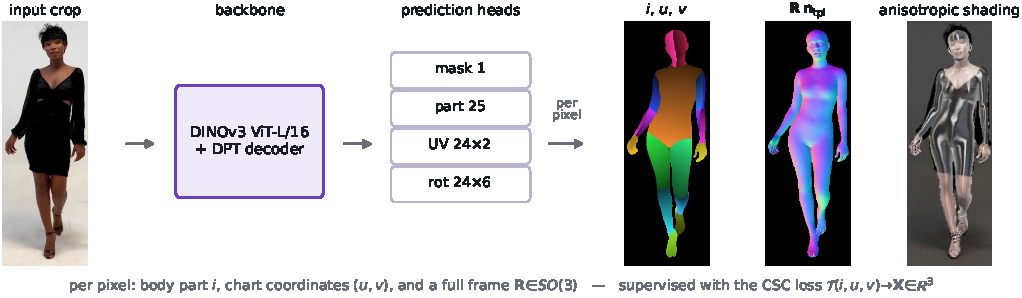
\includegraphics[width=0.58\linewidth]{figs/fig_method.pdf}
\caption{\textbf{Pipeline.} A person crop is encoded by DINOv3 ViT-L/16 and a DPT decoder into
four heads --- body mask, $24$-way part, $24{\times}2$ chart coordinates, $24{\times}6$ rotation ---
read out per pixel as $(\hat\imath,\hat u,\hat v,\hat R)$; correspondence is supervised in metric
template space through the operator $\Phi$ of \cref{sec:csc} and rotation by a chordal loss against
the template's own surface frame.}
\label{fig:method}
\end{figure*}

\subsection{From surface points to surface frames}
\label{sec:task}

Let $T$ be a fixed template (neutral SMPL-X~\cite{pavlakos2019smplx}) partitioned into the $24$
DensePose parts, each with a chart $\mathcal{C}_i\subset[0,1]^2$. The classical task predicts at
every pixel $x$ a body flag $\hat m$, a part $\hat\imath$ and chart coordinates $(\hat u,\hat v)$
--- together a template point $\pi(x)$. We add $\hat R(x)\in SO(3)$, the rotation carrying the
template's \emph{own} surface frame at $\pi(x)$ into the camera-space frame of the posed surface,
so that $\hat R\,\mathbf{n}_T(\pi(x))=\mathbf{n}_{\mathrm{cam}}(x)$ and
$\hat R\,\mathbf{t}=\mathbf{t}_{\mathrm{cam}}(x)$ for \emph{any} template-attached $\mathbf{t}$.
Anchoring to the template rather than the chart matters: a chart-induced tangent frame would flip
at seams, be undefined where the chart degenerates, and change meaning under a re-cut, including
our own. It remains a gauge choice --- fixed by the template's tessellation through
\cref{eq:kabsch} --- but it makes the target \emph{chart-independent} and continuous across part
boundaries, so its ground truth is a per-vertex field. Since $SO(3)$ has no continuous global
three-parameter chart the net emits $g\in\mathbb{R}^6$~\cite{zhou2019continuity}, mapped to
$\psi(g)\in SO(3)$ by Gram--Schmidt.

The backbone is DINOv3 ViT-L/16~\cite{dinov3}: tokens after blocks $\{4,11,17,23\}$ are projected
to $d{=}256$, resampled to $\{4,2,1,0.5\}\times$ the token grid and fused by four DPT
blocks~\cite{ranftl2021dpt}, only the patch embedding frozen ($302$M of $303$M parameters train).
Four heads predict a body mask (BCE over \emph{all} pixels), $24$ parts (cross-entropy on
foreground), $24{\times}2$ chart coordinates (smooth-$L_1$ on the ground-truth part's channels) and
$24{\times}6$ rotation. The $25$-way readout is \emph{factorised} into a binary body head and a
$24$-way part head with no background class, so the part head cannot resolve an ambiguous seam by
predicting background. A per-part rather than shared rotation head buys $0.53^\circ$ of geodesic
error at matched step with synthetic part accuracy and UV error unchanged, but costs $1.8$ COCO AP
points (\cref{tab:recipe}); we ship it and the final recipe recovers the AP. At test time we take
$\hat\imath=\arg\max_i\hat s_i$ where $\hat m>0$ and gather $(\hat u,\hat v)$ and $\hat R$ from
that part, so every COCO number and every end-to-end geodesic error includes part-classification
error; metrics gathered by the ground-truth part are labelled \emph{oracle}. Wherever a per-part
volume is resampled --- as in COCO scoring, on the box expanded by $1.2\times$ --- we resize the
\emph{volume} and gather afterwards, since resizing the gathered map blends adjacent parts.

\subsection{Rotation supervision}
\label{sec:rotsup}

The target $R_v$ is the local as-rigid-as-possible rotation~\cite{sorkine2007arap} of the one-ring
$\mathcal{N}(v)$ between template vertices $\bar V$ and camera-space vertices $V$: a Kabsch
problem~\cite{kabsch1976} with a normal pin, solved by SVD $H_v=U\Sigma W^{\!\top}$,
$R_v=W\,\mathrm{diag}(1,1,\det(WU^{\!\top}))\,U^{\!\top}$, where
\begin{equation}
  H_v \!=\!\!\! \sum_{j \in \mathcal{N}(v)} \!\!\! (\bar V_j \!-\! \bar V_v)(V_j \!-\! V_v)^{\!\top}
      \!\!+ \lambda \Big(\!\!\!\sum_{j \in \mathcal{N}(v)}\!\!\! \lVert \bar V_j \!-\! \bar V_v \rVert^2 \Big)
        \bar n_v n_v^{\!\top}\!,
  \label{eq:kabsch}
\end{equation}
$\lambda{=}25$ and $\bar n_v,n_v$ the area-weighted unit vertex normals. Without the pin this is a
pure edge fit whose third axis is whatever the one-ring implies; the pin pulls it towards the
surface normal, which is what makes the transport identity useful. The pin is \emph{soft}, so that
identity holds only approximately, and we measured neither the residual angle nor the sensitivity
to $\lambda$. The per-pixel label is the barycentric blend of the rasterised face's three vertex
$6$D vectors through $\psi$ --- formally the operation \cref{sec:data} argues against, but at the
scale of one triangle, where the three frames are near-parallel; we rely on that and do not measure
it. Labels come from the \emph{body} surface, so on clothed regions the frame is that of the body
beneath the garment. On the foreground $M$, gathering the ground-truth part's six channels, the
loss is chordal, $|M|^{-1}\sum_x\lVert\psi(\hat
g_{i_{\mathrm{gt}}(x)}(x))-R_{\mathrm{gt}}(x)\rVert_F^2$: since $\lVert
R_1-R_2\rVert_F^2=4(1-\cos\theta)$ it is a monotone surrogate for the geodesic angle $\theta$ that
keeps $\arccos$ out of the graph~\cite{hartley2013rotation}.

\subsection{Fold-free charts}
\label{sec:charts}

The official atlas builds each chart as a planar PCA projection of its part. For the $18$
half-cylinder parts this is injective; for hands and feet it is not, because a hand is \emph{one}
part containing palm, back and fingers, and sampling surface points to count how many of the part's
triangles claim each $(u,v)$ shows roughly $49\%$ of hand and $53\%$ of foot surface non-injective,
at a median $3$D distance of $60$--$67$\,mm between claimants (supp.). We re-flatten those four
parts by splitting each into two \emph{sheets} on the sign of $\langle n_f,n_i\rangle$ --- face
normal against chart-plane normal, i.e.\ palm/back and top/sole --- keeping the original PCA
projection, renormalising within each sheet and packing the sheets into halves of the unit square
with a gutter no bilinear stencil can span; within a sheet the surface is a height field over the
chart plane, so the projection that folded becomes single-valued. This is exact only away from the
rim, where $\langle n_f,n_i\rangle\!\approx\!0$ makes the assignment arbitrary: residual overlap is
$0.0\%$ (hands) and $0.7\%$ (feet), and the split adds a rim seam and a per-sheet scale, neither
measured. The head is left unchanged, its residual being hidden geometry \emph{inside} the part and
identical (${\approx}0.6\%$) in \textsc{v1} and \textsc{v2}, so the atlas is fold-free on hands and
feet and the head is masked, not fixed. Nothing in the model changes: the loader derives
ground-truth UV from the face-UV asset on the fly, so swapping it needs \emph{no} re-sharding
($3.7$\,TB untouched) and $20$ of $24$ charts stay bit-identical. COCO annotations are \textsc{v1},
so a \textsc{v2} model is scored through an exact texel-wise remap, and joint COCO fine-tuning
\emph{skips} the sparse UV term on parts $3$--$6$ while keeping their part cross-entropy, because
COCO's UV labels there are \textsc{v1} and \textsc{v1} is fold-ambiguous there anyway.

\subsection{Canonical surface coordinates}
\label{sec:csc}

Three properties of the atlas make a smooth-$L_1$ on $(u,v)$ a poor objective: charts are
renormalised by their own PCA span and spans differ $8\times$; $(u,v)$ jumps at seams where the
surface does not, and $6.1\%$ of template vertices touch more than one chart; and a pointwise loss
constrains the value of the correspondence map but not its spatial derivative, the local geometry
any consumer of a frame reads --- we offer this third one as motivation, not measurement. We
therefore bake, per part, a $512^2$ texture $T_i$ of template XYZ over that part's chart by
barycentric rasterisation and read it as $\Phi(i,u,v)=\mathrm{bilinear}(T_i,(u,v))$ with one 3D
\texttt{grid\_sample} whose part axis lands on slice centres, so part selection is exact and $\Phi$
is differentiable in $(u,v)$ with an exact analytic Jacobian. Against exact barycentric XYZ on
$200$k surface points, on the $74.5\%$ an ambiguity mask admits, median error is below $0.001$\,mm
and p99 is $0.335$\,mm, but the maximum is $63$\,mm on sliver triangles, so our own $\max<1$\,mm
criterion fails: $\Phi$ is exact for the overwhelming majority of the surface and \emph{not}
uniformly so, and we accept that tail rather than claim it away, because the losses are $L_1$
averages over millions of pixels (supp.). With $\hat X(x)=\Phi(i(x),\hat u_{i(x)}(x),\hat
v_{i(x)}(x))$,
\begin{align}
  \mathcal{L}_{\mathrm{xyz}}
    &= \tfrac{1}{3|M'|} \! \sum_{x \in M'} \! \big\lVert \hat X(x) - X_{\mathrm{gt}}(x) \big\rVert_1
    \;\text{[m]}, \label{eq:lxyz}\\
  \mathcal{L}_{\mathrm{grad}}
   &= \tfrac{1}{N} \sum_{s,d} \tfrac{1}{3|E_d^{(s)}|} \!\! \sum_{x \in E_d^{(s)}} \!\!
     \big\lVert \kappa_c(\Delta_d \hat X^{(s)}) - \kappa_c(\Delta_d X^{(s)}_{\mathrm{gt}}) \big\rVert_1 ,
  \label{eq:lgrad}
\end{align}
the second multi-scale gradient
matching~\cite{eigen2015multiscale,li2018megadepth,ranftl2020midas} on correspondences rather than
depth, over $S{=}4$ scales and axes $d\in\{u,v\}$, with $E_d^{(s)}$ the edges \emph{both} of whose
endpoints are valid and $\kappa_c$ clipping each coordinate to $\pm c{=}0.20$\,m/px. Both sides are
clipped, so \cref{eq:lgrad} is deliberately blind to steps larger than $c$, keeping ${\sim}0.5$\,m
self-occlusion jumps from dominating a term meant to shape smooth structure; at $c{=}0.05$ it goes
blind to the blur it exists to remove. With $M$ the foreground minus hidden faces we keep only
pixels where the chart reproduces the pixel's own known $3$D point,
\begin{equation}
  M' \!=\! M \cap \Big\{ x : \big\lVert \Phi\big(i_{\mathrm{gt}},u_{\mathrm{gt}},v_{\mathrm{gt}}\big)(x)
       - X_{\mathrm{gt}}(x) \big\rVert_2 < \tau \Big\},\; \tau{=}5\,\mathrm{mm}.
  \label{eq:valid}
\end{equation}
The test is exact rather than heuristic because $i_{\mathrm{gt}}$, $(u,v)_{\mathrm{gt}}$ and
$X_{\mathrm{gt}}$ derive from the \emph{same} rasterised face and barycentrics, so every pixel
knows its own true template point and the loss can simply ask the chart to reproduce it; where the
chart folds or covers hidden geometry it fails and the pixel drops, so the fold mask falls out of
the construction rather than being hand-tuned. We never logged $|M'|/|M|$, so the fraction of
foreground receiving metric supervision is unmeasured; $\hat u$ is gathered by the ground-truth
part, one of three variants (\cref{sec:exp_csc}). The objective adds $\mathcal{L}_{\mathrm{mask}}$,
$\mathcal{L}_{\mathrm{part}}$, $\mathcal{L}_{\mathrm{uv}}$ and $\mathcal{L}_{\mathrm{rot}}$ at
weight $1$ to $\mathcal{L}_{\mathrm{xyz}}$ at $2$ and $\mathcal{L}_{\mathrm{grad}}$ at $5$.

\subsection{Training data and label integrity}
\label{sec:data}

We train on BEDLAM2~\cite{tesch2025bedlam2} for clean single-person coverage and
MAMMA-syn~\cite{cuevas2025mamma} for multi-person contact, mixed ${\approx}50/50$. Because MAMMA is
our evidence that occlusion supervision transfers, we hold out \emph{sequences}, not frames:
$\mathrm{md5}(\text{seq})\bmod50=0$ selects $29$ of $2211$ sequences ($59$ of $5417$ shards) across
all four sub-datasets, and shard names embed sequence ids, so the exclusion is exact.

The faithful DensePose loss never resamples labels, and with a rotation field the cost of breaking
that rule is measurable: bilinearly resizing a $6$D field \emph{averages the rotations of two
different surfaces} wherever a limb occludes the torso, and Gram--Schmidt of that blend is a frame
belonging to neither --- on MAMMA at $832\!\rightarrow\!384$, $4.4\%$ of labels are wrong by more
than $10^\circ$ and $3.2\%$ by more than $30^\circ$, up to a $180^\circ$ flip, concentrated at
exactly the occlusion boundaries the occlusion data exists to teach. We therefore rasterise ground
truth once into a fixed $512^2$ canvas ($1.2\times$ the tight body box) and never touch it again,
warping the \emph{prediction} into it with one closed-form \texttt{grid\_sample} per head:
\emph{the direction is the argument}, since a network output is a smooth field that warping merely
\emph{evaluates} at the ground truth's pixel centres, whereas the ground truth has true
discontinuities that warping destroys. Because the canvas is fixed-size the loss also stacks, so
every head, including the $144$-channel rotation field, is supervised at full $512^2$; crops stay
concentric with scale jitter $1.25$--$1.4\times$, and horizontal flip is disabled whenever the
rotation head is active, since a mirrored rotation ground truth is not implemented. SMPL-X also
carries geometry never visible yet still winning rasterisation --- eyeballs, mouth cavity, inner
lips and eye sockets, $3870$ of $20\,908$ faces, $0.106\%$ of foreground --- whose labels are coin
flips; the loader fills the part map first and \emph{then} clears the foreground gate there, so
part, UV, rotation and CSC skip those pixels while the body-mask BCE still sees the whole person.
We optimise with AdamW under layer-wise learning-rate decay (LLRD; $26$ groups, embeddings at
$\text{lr}\cdot0.75^{25}$), grad-clip $1.0$, $500$-step warmup, cosine schedule, batch $32$ per GPU
on $4{\times}$GH200, colour jitter the only further augmentation. The base rate is
$3{\times}10^{-4}$; $10^{-3}$ is the synthetic optimum but costs $3.4$ COCO AP points
(\cref{tab:recipe}). Training is two-stage: $120$k steps on the synthetic mix, then a $10$k-step
joint fine-tune (flat $5{\times}10^{-5}$, half the batches from
DensePose-COCO~\cite{guler2018densepose,lin2014coco} under the sparse loss above), saving every
$1$k steps; selection is discussed in \cref{sec:exp_main}.
